%# -*- coding: utf-8-unix -*-
%%==================================================
%% chapter03.tex
%%==================================================

%\bibliographystyle{sjtu2}%[此处用于每章都生产参考文献]
\chapter{需求分析}
\label{chap:requirement}
本系统分为3个共享数据库的互相关联又相对独立的模块,需求分析的工作不是仅仅做三遍就行,而是要考虑到相互联系和共用资源。由于整体上是传感器管理系统,所以传感器(Sensor)这个资源肯定是共享的,不同的系统都得有登录和权限管理,所以用户(User)也需要共享,这两种资源需要统一在版本管理系统中管理,这样能够保证所有用户和设备资源的一致性,又能在此基础上各自独立地实现业务逻辑。不同系统上的用户可能实际含义不太相同,本系统使用用户的角色(role)属性来区分,具体角色有:
\begin{description}
  \item[普通用户(user)] Smart Home模块和Smart City模块的最终用户,一个传感器会属于一个普通用户,一个普通用户可以拥有多个传感器。
  \item[管理员(admin)] 版本管理模块的最终用户,也就是Clarity的硬件开发人员和管理人员,除了管理传感器版本等信息外还可以管理用户。
  \item[根用户(root)] 超级用户,给系统维护人员或开发人员的角色,拥有最高权限,可以修改任何资源。
\end{description}

注1:本系统中版本管理模块取名“balanar”,Smart Home取名“robotic”,Smart City名字叫“azwraith”。这3个名字都只做内部代号,但也许会在一些代码或截图中出现,为免误解,特此声明。其中只有robotic(意为机器人的)跟项目内容有点联系,其余两个无实际含义。

注2:本章节中的原型和设计稿都不一定与最终的需求吻合,因为可能有些需求修改没有必要在原型和设计稿上体现。

下面本章将详细从不同的角度对各模块进行需求分析:
\section{版本管理模块}
本模块的主要用户是硬件开发人员,原本用户使用Excel记录传感器版本、批次、拥有者等信息,但随着传感器的不断改进,合作方越来越多,制作给合作方的特殊版本越来越多,零件进货的批次各有不同,使用Excel的时间成本和精力成本越来越高。
\subsection{功能需求}
所以版本管理模块需要解决的问题和实现的功能如下:
\begin{enumerate}
  \item 版本、批次和传感器之间的关系混乱,包括硬件版本、固件版本、软件版本、五种零件版本和五种零件批次;Balanar要理清关联关系,用最佳的数据结构体现;
  \item 版本编号格式难以维护;Balanar要能够自动校验格式并给出错误描述;
  \item 硬件版本和固件版本兼容,固件版本又和软件版本兼容;Balanar要能够记录和判断版本兼容性;
\end{enumerate}
\subsection{用户用例}
经过与需求方的多次需求会议,本课题总结出如下用户用例:
\begin{enumerate}
  \item 每当用户(这里用户指Clarity的硬件开发人员)设计出新版本的零件,需要到系统中添加一个零件版本,填写一些参数。
  \item 每当用户下单订购或者收到一批零件,需要到系统中添加一个零件批次或者修改到货日期,选择相应的一种零件版本。
  \item 每当用户准备装配一种拥有新版本零件的传感器,需要到系统中添加一个硬件版本,选择相应的五种零件版本。
  \item 每当用户准备装配一种拥有新固件的传感器,需要到系统中添加一个固件版本,并添加对应的兼容性。
  \item 每当用户装配完成一批新的传感器,需要到系统中添加这些传感器,选择相应的硬件版本、固件版本和五个零件批次,同时可以指定一个拥有者(普通用户)。
  \item 每当Clarity有新的合作伙伴,Clarity的管理人员可以添加普通用户(角色),将来有给他们专用的传感器时,可以指定为拥有者。
\end{enumerate}
\subsection{数据模型}
本课题使用ARIS业务流程建模软件建立了一个数据模型,如图3-1所示,其中灰色的Sales是不在本模块也不在本系统中的:
\begin{figure}[H]
 \centering
 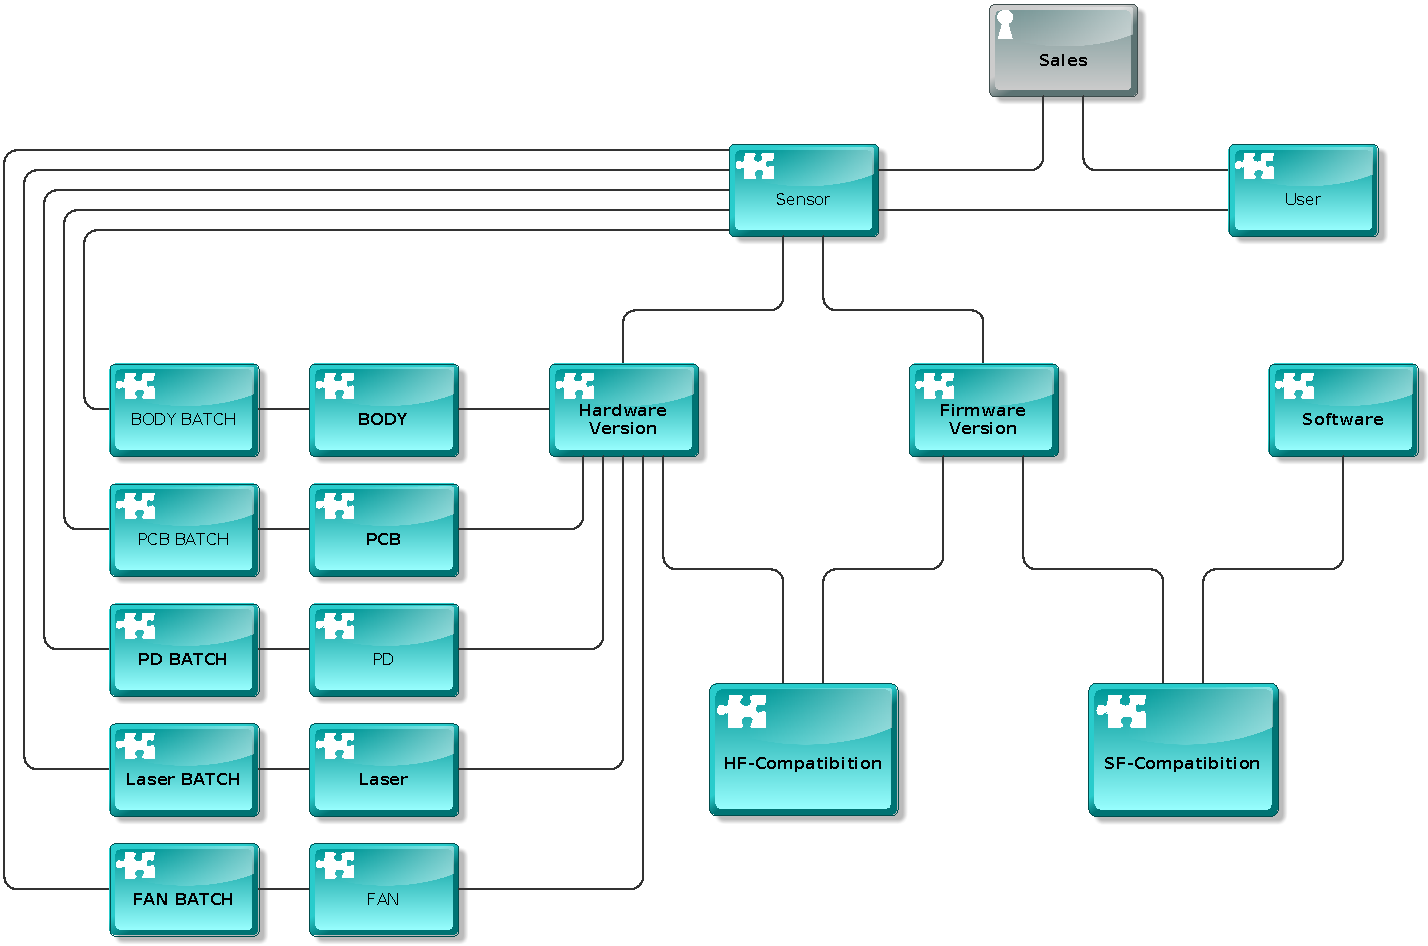
\includegraphics[width=0.8\textwidth]{data_model.png}
 \bicaption[fig:balanar_data_model]{版本管理模块 数据模型}{版本管理模块 数据模型}{Fig}{Version Management module's data model}
\end{figure}

\subsection{数据字典}
本课题使用普通文本定义了一套数据字典,以免开发过程中混淆不同的资源名和属性名,同时对字段类型做了一些限定,这里只展示了开头部分关于传感器资源的定义,详情请看附录A(数据字典)。
\begin{lstlisting}[language={JSON}, caption={版本管理模块的数据字典}]
Explanation:
@: description or restriction of keys or attributes
@fk: short for 'foreign key'
@pk: short for 'primary key'
@uk: short for 'unique key'
@path(type): a file or directory path in cdn of specific type
...: a combination of object, e.g. {a, b, ...{c, d}, e} == {a, b, c, d, e}
': {}': attributes of a table or an attribute
': type()': describe type of an attribute, including [string, integer, decimal, enum]
---------------------------Tables---------------------------
Sensor: {
  @pk id
  @fk hardwareVersion
  @fk firmwareVersion,
  @fk componentBatches: {body, pcb, photodiode, laser, fan},

  threshold: type(integer),
  noiseLevel,
  calibrations: {
    mass: type(decimal),
    number: type(decimal)
  },
  applicationType: type(enum(SMART_CITY)),
}
\end{lstlisting}

\subsection{快速原型}
本系统在正式开发之前还使用一款叫做balsamiq模拟软件做了一个快速原型。如图3-2所示,这里只展示了一个页面,详情请看附录B(快速原型)。
\begin{figure}[!htp]
 \centering
 \includegraphics[width=0.8\textwidth,page=8]{pdf/balanar_prototype.pdf}
 \bicaption[fig:balanar_mockup]{版本管理模块原型样例}{版本管理模块原型样例}{Fig}{Example of Version Management module’s mockups}
\end{figure}

\section{Smart Home模块}
本模块的当前的主要目标客户是一家日本的家电制造企业,最终用户是该企业家电产品的用户。该企业生产的产品是空调和空气净化器等家用电器,因此Clarity为其量身打造了智能家居(Smart Home)解决方案。
\subsection{智能家居解决方案}
首先,目标用户是购买了该企业各种家电和空气净化器的个人或家庭,用户还可以随身携带一个Clarity的个人空气质量传感器。普通的空气净化器只能一直开着或者在人的操控下间歇性地净化空气,而搭载空气质量传感器的家电也只能检测空气质量并报告给用户,并不能实际改善空气质量,Clarity在两者之间引入了一个烧录了智能程序的可编程扫地机器人巧妙地弥补了两者的不足。此智能家居解决方案按以下流程工作:
\begin{enumerate}
  \item 不同房间的空气质量传感器持续上传数据到服务器,服务器保存数据;
  \item 服务器定时地计算并评估空气质量的好坏;
  \item 一旦有房间空气质量低于一定水平,服务器就会给机器人下达净化指令,机器人会移动到对应的房间并开启其上搭载空气净化器;
  \item 空气质量好转之后,服务器再给机器人下达停止指令,机器人会关掉空气净化器原地待命;
\end{enumerate}
\subsection{功能需求}
\begin{enumerate}
  \item 实时展示个人、家里和城市的空气质量情况和健康评价;
  \item 实时展示家里不同房间的空气质量状况;
  \item 实时展示机器人的位置和空气净化器的工作状态;
  \item 能够绘制每个房间的历史空气质量折线图;
  \item 能够让用户手动控制机器人;
\end{enumerate}

\subsection{用户用例}
\begin{enumerate}
  \item 用户随时查看功能需求中展示的所有实时信息;
  \item 用户想要手动控制机器人时,可以调节到手动模式;
  \item 用户可以控制机器人去任何房间并自动开始净化空气;
\end{enumerate}
\subsection{设计稿}
本模块的需求方给出了一个比较详细的设计稿,如图3-3所示,这里只展示了一个页面,详情请看附录C(设计稿)。
\begin{figure}[H]
 \centering
 \includegraphics[height=0.8\linewidth, page=2, angle=-90]{pdf/robotic_design.pdf}
 \bicaption[fig:smart_home_design]{Smart Home模块设计稿样例}{Smart Home模块设计稿样例}{Fig}{Example of Smart Home module’s design}
\end{figure}

\section{Smart City模块}
本模块的当前主要目标客户是美国一家城市政府,最终用户是政府工作人员。该城市计划大量安装Clarity的传感器以监控城市空气质量,这就需要在智慧城市级别提供空气质量的数据查看和设备管理服务。
\subsection{功能目标}
本模块需要提供一下功能:
\begin{enumerate}
  \item 能够添加和删除、显示和隐藏设备(传感器);
  \item 以地图形式直观的展示传感器位置和当前空气质量;
  \item 以图表形式直观地展示某些设备的最近历史数据,
  \item 以csv形式提供不同设备、时间跨度、时间精度和空气质量度量\footnote{如AQI或者pm2.5浓度}的空气质量数据;
\end{enumerate}

\subsection{用户用例}
\begin{enumerate}
  \item 市政部门安装了新的传感器或者拆除了旧的传感器,需要在此系统上添加或删除设备。
  \item 政府工作人员随时查看设备列表、传感器位置和历史数据。
  \item 政府工作人员想要下载某几个设备的最近历史数据,可以在设备列表上选择一些设备,在图表中选择时间精度和度量,然后在图表的工具栏中点击下载。
  \item 政府工作人员想要下载某一个设备的长期历史数据,可以在一个单独的下载页面上,在表单中选择时间跨度、时间精度和度量,然后点击下载。
\end{enumerate}

\subsection{快速原型}
本系统在开发之初做了一个简单的快速原型,如图3-4所示。
\begin{figure}[!htp]
 \centering
 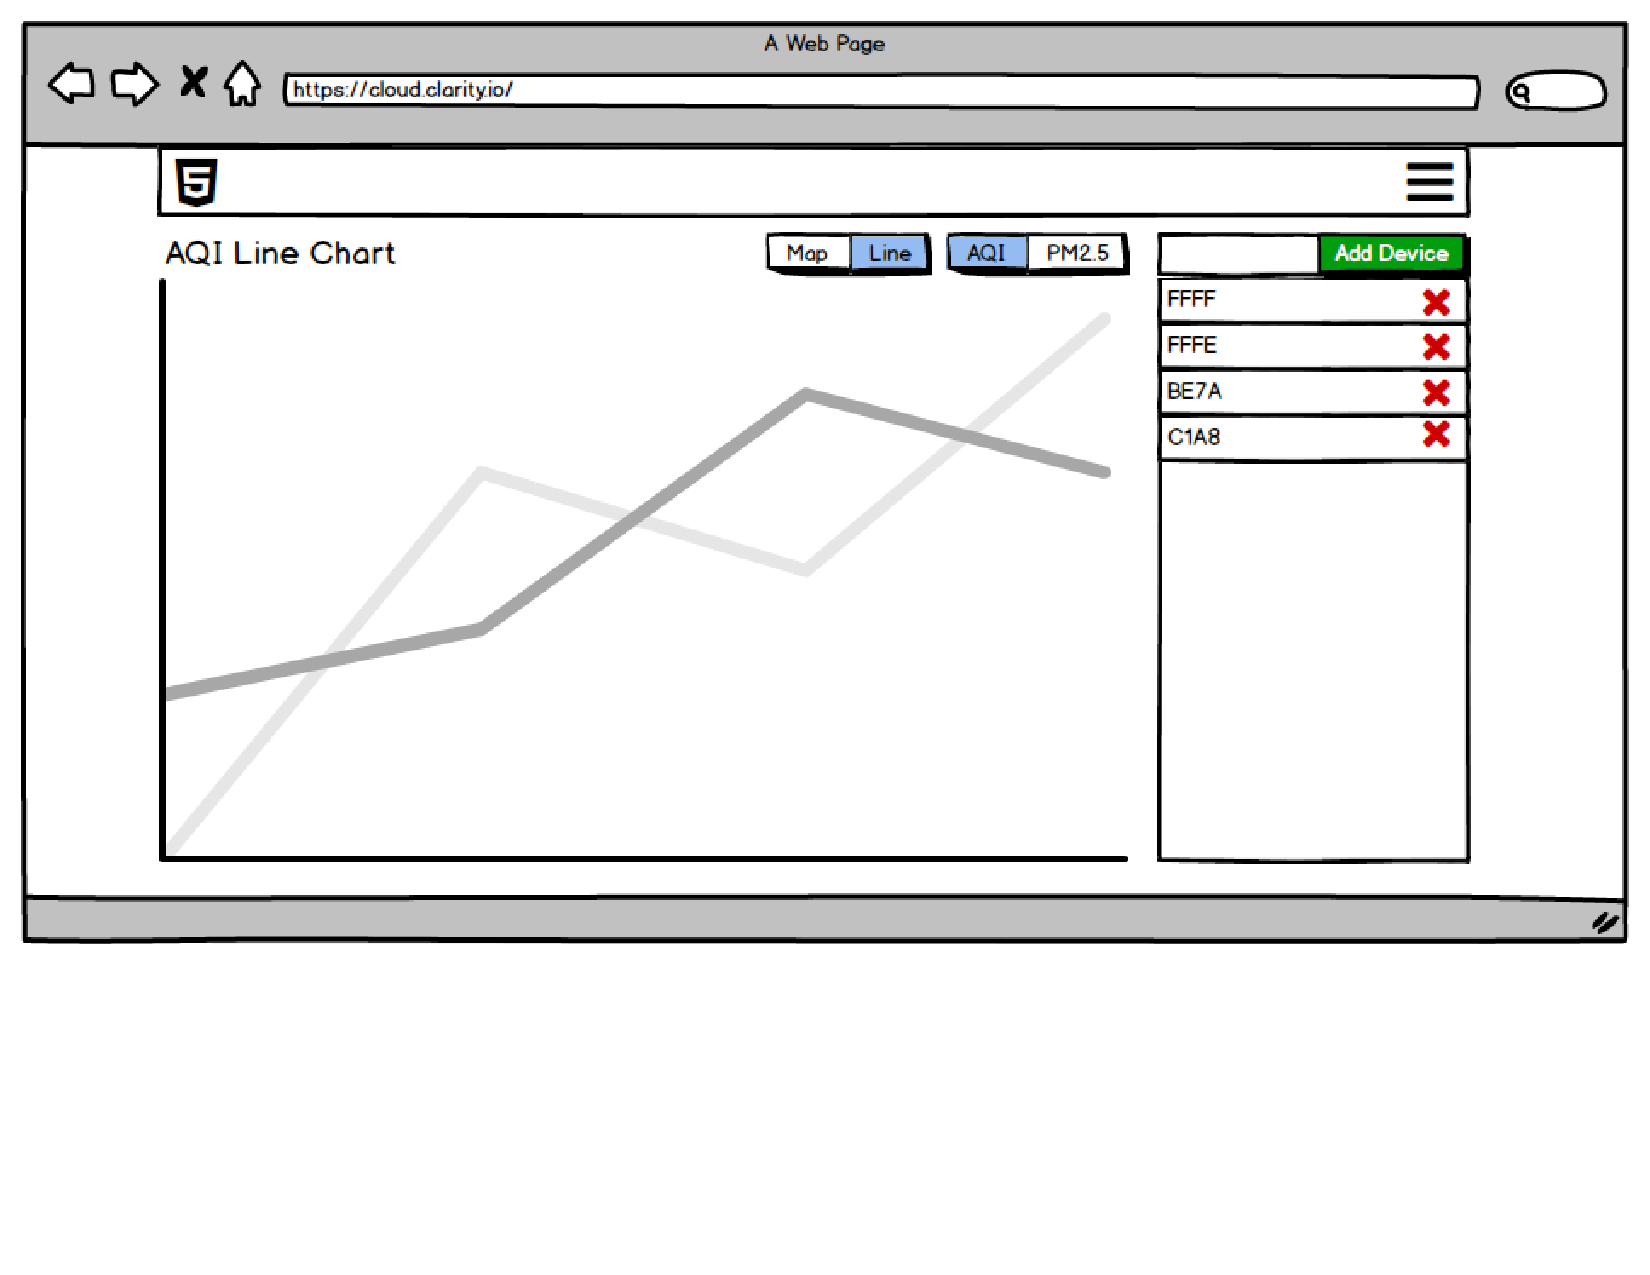
\includegraphics[width=0.8\textwidth]{pdf/azwraith_prototype.pdf}
 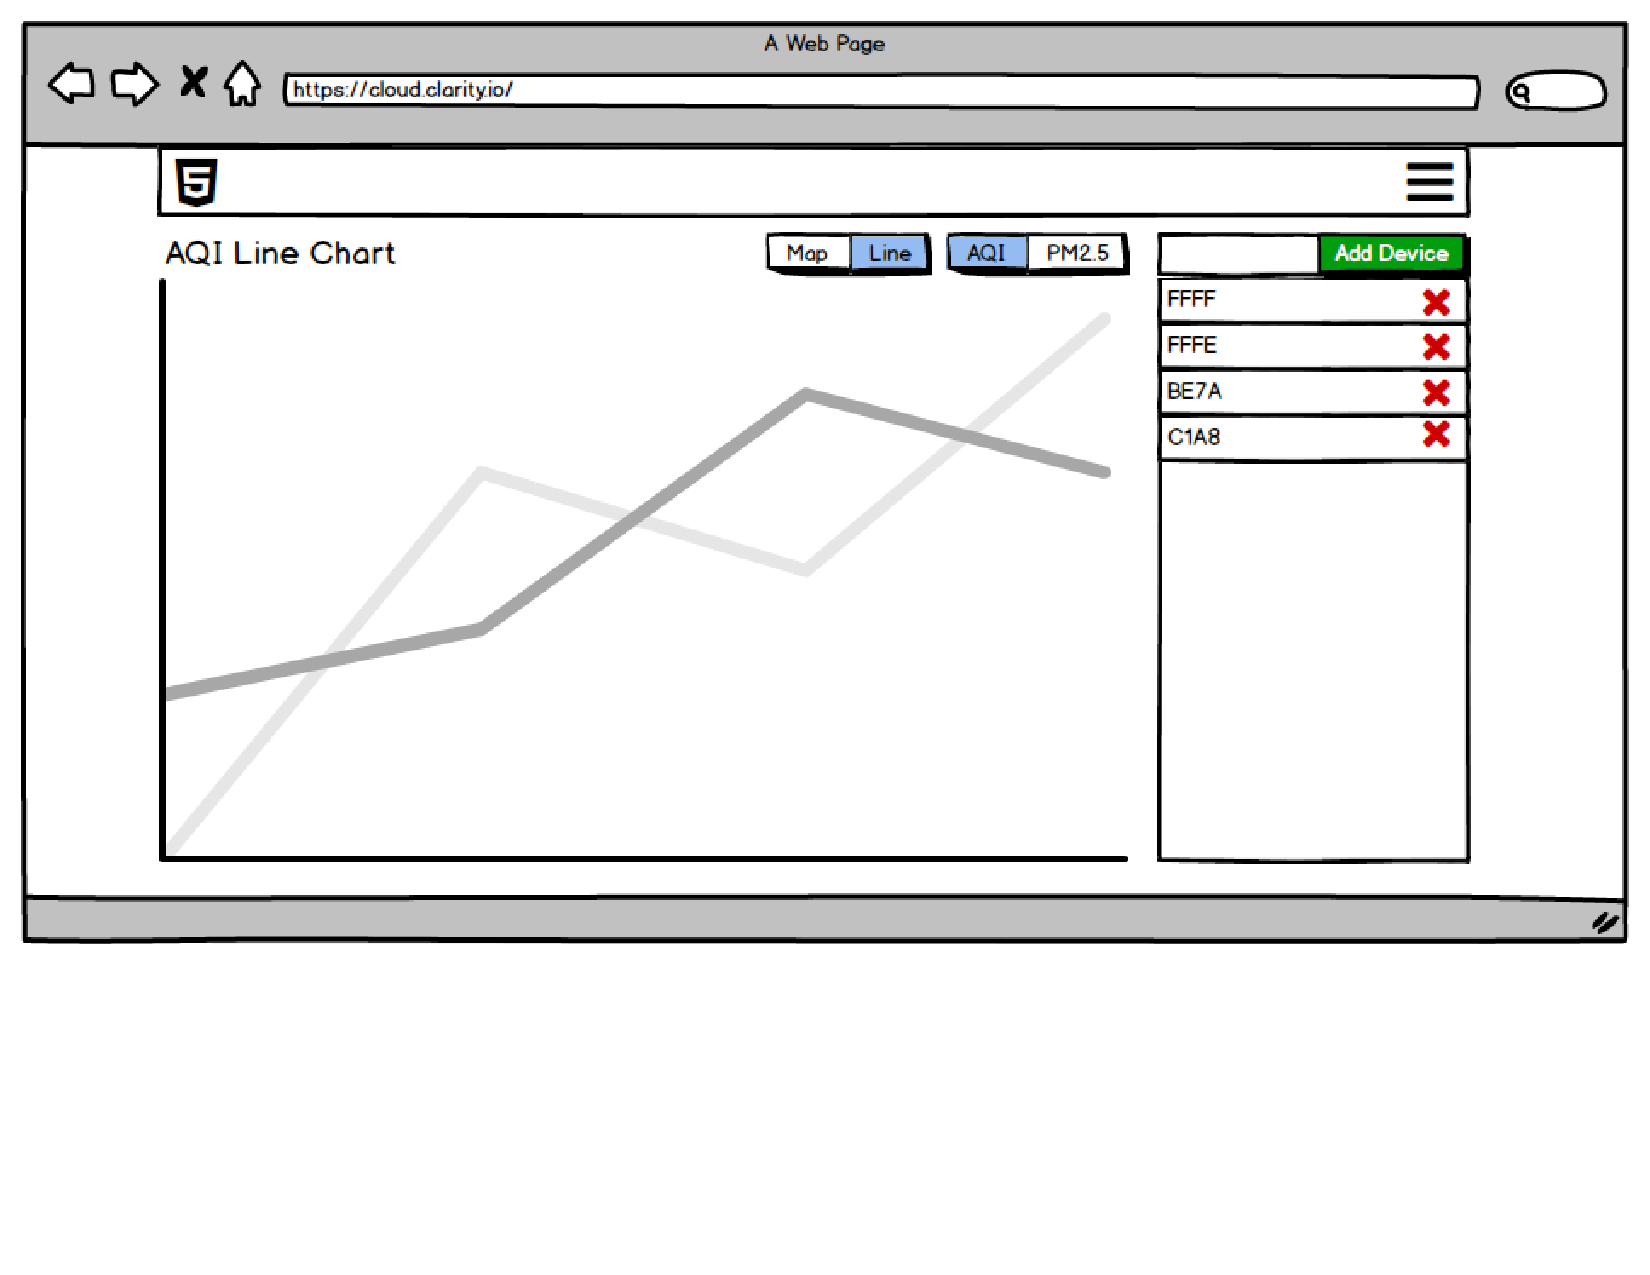
\includegraphics[width=0.8\textwidth]{pdf/azwraith_prototype.pdf}
 \bicaption[fig:azwraith_mockup_1]{Smart City模块原型}{Smart City模块原型}{Fig}{Smart City module’s mockups}
\end{figure}

\subsection{设计稿}
但后来因为这个模块比较重要,而且不像版本管理模块不是非常注重UI,公司又请专门的设计师给出了一个设计稿,如图3-5所示。
\begin{figure}[htb]
 \centering
 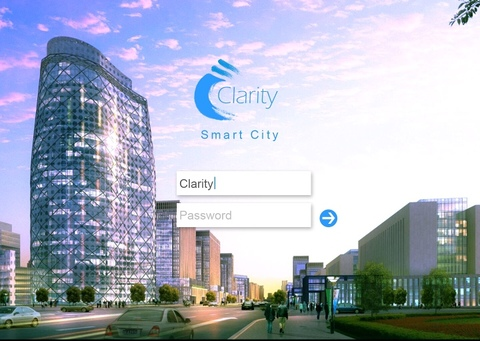
\includegraphics[width=0.8\linewidth]{azwraith_login.jpg}
 
 \vspace{0.5cm}
 
 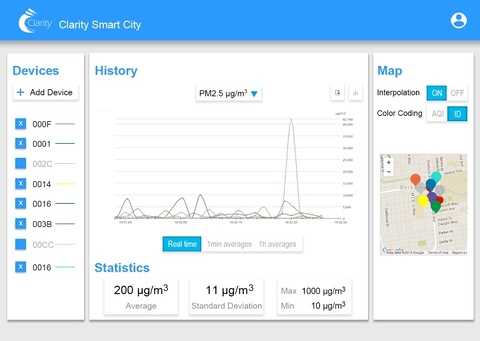
\includegraphics[width=0.8\linewidth]{azwraith_smart_city.jpg}
 \bicaption[fig:azwraith_login]{Smart City模块登录设计稿}{Smart City模块设计稿}{Fig}{Designs of Smart City module}
\end{figure}

